%% LyX 2.3.2-2 created this file.  For more info, see http://www.lyx.org/.
%% Do not edit unless you really know what you are doing.
\documentclass[english]{article}
\usepackage[T1]{fontenc}
\usepackage[utf8]{inputenc}
\usepackage{babel}
\usepackage{amsmath}
\usepackage{amsthm}
\usepackage{amssymb}
\usepackage{graphicx}
\usepackage[unicode=true,pdfusetitle,
 bookmarks=true,bookmarksnumbered=false,bookmarksopen=false,
 breaklinks=false,pdfborder={0 0 1},backref=false,colorlinks=false]
 {hyperref}

\makeatletter

%%%%%%%%%%%%%%%%%%%%%%%%%%%%%% LyX specific LaTeX commands.
%% Because html converters don't know tabularnewline
\providecommand{\tabularnewline}{\\}

\makeatother

\begin{document}
\title{Tennis Match as Random Walk with Memory: Application to Grand Slam
Matches Modelling}
\author{Tomáš Kouřim$^{1,2}$, Petr Volf$^{2}$ \\
 $^{1}$ Faculty of Nuclear Sciences and Physical Engineering, \\
Czech Technical University in Prague\\
 $^{2}$Institute of Information Theory and Automation,\\
 Academy of Sciences of the Czech Republic}
\maketitle
\begin{abstract}
The contribution introduces a Bernoulli-like random walk with transition
probabilities depending of its recent steps. Then, implicitly, the
walk depends on the walk whole history. The main objective is its
application to modelling and then to prediction of tennis matches.
The data are taken from the Grand Slam tennis matches, since 2009
till 2019. The flexibility of the model is tested thoroughly on several
datasets selections and the results reported. It is shown that the
model corresponds well to the majority of matches. Finally, the model
is also used for the in-play betting, with rather encouraging results.

\textbf{\emph{Key words:}} Random walk, transitions dependent on history,
tennis modelling, prediction, betting
\end{abstract}

\section{Introduction}

Tennis is one of the oldest and most traditional sports, which is
pursued worldwide and on all possible levels. It is an industry that
operates with billions of dollars every year. It is therefore no wonder
that even in such a traditional sport as tennis there are always new
methods and technologies introduced. Computer imaging is used in the
hawk-eye technology helping to determine whether a ball was out, material
science allows to manufacture better and better rackets and other
equipment, medicine science develops new methods of effective training
etc. Mathematics is becoming a very important part of tennis as well
as it can produce models simulating game situations and predicting
their probabilities. This can be useful for the trainers who can use
such models to better prepare their players for their matches, but
most of all it is used for sports betting. The market of sports betting
is despite strict regulations continuously growing both in revenues
as in profits. It is therefore no wonder that the demand for accurate
sports models, including the tennis, is tremendous.

There are several different approaches in modelling and simulating
tennis games. The most common ones use Markov chains as the baseline
of the model, creating Markov-like chains usually from one particular
part of the game - set by set, game by game, point by point or even
rally by rally \cite{barnett2005combining,hunter2009can,newton2009monte,spanias2012predicting}.
Other approaches use some sort of regression (logistic, probit) \cite{del2010differences},
\cite{dziedzic2015predicting,klaassen2003forecasting}. The methods
can be also divided into those focusing on the match result itself
\cite{dziedzic2015predicting,klaassen2003forecasting}, those focusing
on the modelling the match development (already mentioned methods
using random processes models), and also concentrated to partial results
during a match - in play probabilities \cite{hunter2009can}. Comparison
of some of the existing methods can be found in Kovalchik \cite{kovalchik2015comparative}.
In this paper a task is to find the best prediction way. However,
to reach good results is not a matter of model only, it is also a
matter of information used. This problem has been discussed also in
\cite{ja2016ddny}.

Thus, a basic information is the rating of players. However, a number
of other data is as a rule available concerning each particular match.
For instance the past performance, match conditions (the surface,
location) and even the bookmaker's odds, which are in fact constructed
from all the information considered to be relevant. And the goal of
every modelling tool should be to do better (at least sometimes) than
the prediction based on them (and, eventually, to use them as a partial
information source).

The present contribution describes the tennis match using a random
walk model, not insisting on its Markov property. The match in fact
consists of several such processes. A series of sets within a match,
games within a set, points within a game or even strokes within a
point can be all considered a random process and modelled using a
random walk. These walks are well described by the tennis rules and
there exist lots of data describing these random processes (i.e. various
tennis result databases provided by the tennis federation as well
as many private subjects). An analysis of non-Markov development in
tennis matches has been provided already in \cite{ja2015ddny}. In
the present paper, the random walk consisting of a sequence of sets
within a match is studied. Matches played as a best-of-five, i.e.
the men Grand Slam tournaments, are considered. In these matches,
up to 5 steps of the random walk can be observed. The contribution
presents a new version of random walk model with varying transition
probabilities implicitly depending on the history of the walk. The
transition probabilities are altered according to the last one or
two steps of the walk using a memory parameter to either reward or
punish success by increasing or decreasing its probability in the
next step. It seems more than suitable to model tennis matches as
the data suggest that a success in tennis yields another success,
or in other words, that winning one particular part of the match increases
the chances of winning the next part as well. This behavior is well
described by introduced random walk model.

The remainder of the paper is organized as follows: First, the model
of Bernoulii-like random walk with transitions dependent on preceding
steps is introduced. The rest of the paper then deals with its application
to modelling tennis matches. In Section 3 the data are described,
in Sect. 4 the model is evaluated and its flexibility tested. Finally,
the usefulness of the model is assessed also via its use to betting.

\section{Models of random walk with memory}

A basic type of a discrete time random walk is the Bernoulli walk,
with random steps (denote them $X_{i}$ at stage $i$) $X_{i}=\pm1$,
with constant $P(X_{i}=1)=p_{0}$. It is a representation of a Markov
chain, i.e. a memory-less random process. It may fit perfectly to
many real processes, however, many others, including the process of
tennis match development, are more complex, and a memory element has
to be introduced in order to correctly describe them. Then $p_{0}$
can be regarded as based on initial match conditions, and transition
probabilities evolve in dependence on the match state as well as on
its (recent) history.

Naturally, the idea of process transitions depending on the history
of process itself is not new. A rich field of inspiration is for instance
the statistical modelling of recurrent events in the lifetime analysis.
Let us mention for instance the continuous time hazard rate models
as in \cite{percy2007scheduling} with the hazard rate changing after
each event, here implemented to the Cox regression model framework.
As the case analyzed in the present paper is simpler, the time is
discrete and the history is not long, we shall not consider a regression
model (though the use of logistic regression is a natural generalization
here) and change the transition probabilities just by multiplying
them by a convenient parameter. An inspiration to such a modification
of Bernoulli random walk can be found in several papers where the
length of step was changed in a similar way. Thus, Loic Turban in
\cite{turban2010random} presented a model of a one-dimensional random
walk with memory introduced through varying step size. In the paper,
it is assumed that the step size in the direction of the last step
will be lowered by a coefficient $\lambda$ and the step in the opposite
direction will be prolonged so that the sum of absolute values of
the steps remains constant and equal to $2$. The goal is to stabilize
the process. Another interesting variant of model is due Schaltz and
Trimper \cite{schutz2004elephants} introducing a special type of
random walk with the random increment at time step $t$ depending
on the full history of the process, which they compared to an elephant
an its memory. The walk tends to repeat "good decisions" (i.e. steps)
from history and, on the contrary, to avoid repetition of others.
The present application does not allow for changing the steps length,
instead we are changing the transition probabilities in a similar
manner.

\subsection{Transition probabilities dependent on process history}

The concept of the model has been introduced in \cite{ja2017ddny}.
It is also based on the standard random walk with steps $X_{i}=\pm1,i=1,2,...$.
The distribution of the first random variable $X_{1}$ is given by
a starting parameter $p_{0}\in[0,\,1]$, so that $P(X_{1}=1)=p_{0}$
and $P(X_{1}=-1)=1-p_{0}$. After the $i$-th step (for $i\ge1$),
the probability distribution of the next step, $X_{i+1}$, is given
by the (random) probability $p_{i}$, which depends on a coefficient
$\lambda\in[0,\,1]$ and the last random variable $X_{i},\,i=1,2,...$:
\[
p_{i}=\lambda p_{i-1}\,\,\mbox{for}\,\,X_{i}=1,
\]
\[
p_{i}=1-\lambda(1-p_{i-1})\,\,\mbox{for}\,\,X_{i}=-1,
\]
which yields that 
\[
p_{i}=\lambda p_{i-1}+\frac{1}{2}(1-\lambda)(1-X_{i}).\eqno{(1)}
\]
The case $\lambda=1$ corresponds to the standard Markov random walk
with constant transition probability, with $\lambda=0$ the walk would
be a series of alternating steps to the left and right with only the
first step direction being chosen randomly. Therefore only $\lambda\in(0,\,1)$
is further considered. As after the "success" $X_{i}=1$ its probability
in the next step decreases, we can call this scheme a "success punished"
model. Naturally, the opposite, a "success rewarded" variant, is
possible, which leads to a similar expression for $\bar{p}_{i}=1-p_{i}$:
\[
\bar{p}_{i}=\lambda\bar{p}_{i-1}+\frac{1}{2}(1-\lambda)(1-X_{i})\eqno{(2)}
\]
for $i=1,2,...$.

Another alternative is a random walk with each event influencing the
further development of the walk differently, which can be defined
as: Let $\lambda_{0},\,\lambda_{1}\in(0,\,1)$, then 
\[
p_{i}=\frac{1}{2}[(1+X_{i})\lambda_{0}p_{i-1}+(1-X_{i})(1-\lambda_{1}(1-p_{i-1}))],\eqno{(3)}
\]
or a similar model for parameters $\bar{p}_{i}=1-p_{i}$.

In the study \cite{ja2017ddny} the behavior of proposed random walks
types was analyzed, mainly their tendencies after many steps (i.e.
asymptotic properties). As in the present application the walk consists
in just a small number of steps, the long-run properties overview
is omitted here. The main concern is therefore the assessing the initial
probability $p_{0}$ and reliable estimation of parameters $\lambda$.
Another task is to recognize which type of model is the most convenient,
how long history of match is relevant to reliable match development
prediction. In the context of the application to tennis match modelling
(its sets or games as well), in fact the dependence on the last one
step is quite satisfactory. Naturally, there are generalizations which
also could be considered. Except already mentioned regression models
(for instance $\lambda$ depending on available covariates, in a logistic
manner) also models with time-varying parameters can be considered.
In the following real data analysis we select a "success rewarded"
model variant, showing their usefulness and good predictive properties,
also via simulated/real betting, the others (as the regression models)
will be a matter of future research.

\section{Data description\label{sec:Data-description}}

Two datasets were acquired for the purpose of this paper, one for
model development and the other for model testing. The development
dataset contains the results from all Grand Slam tournaments from
2009 to 2018 and corresponding Pinnacle Sports bookmaker's odds (Pinnacle
Sports bookmaker was chosen as it is considered leading in the sports
betting industry). It was created using data publicly available from
website www.oddsportal.com. Every year 4 Grand Slam tournaments (i.e.
Australian Open, French Open, The Wimbledon and US Open) are played,
making it 40 tournaments during the selected period. Each Grand Slam
has $128$ participants in the men singles category played in a single-elimination
system (i.e. $127$ games per tournament). Thus, there were $5080$
matches available altogether. Some matches were not finished due to
one of the players forfeiting and such matches were omitted from the
dataset. Matches without bookmaker's odds were omitted as well. The
dataset contains $4255$ matches with complete data available, played
$432$ players in total. The most active player was Novak Djokovic,
who participated in $188$ matches. On average, each player played
$19.7$ matches, with the median value of $8$ matches played. The
most common result was 3:0, occurring $2138$ times, on the other
hand, 5 sets were played only $808$ times.

The order in which the players are listed is rather random. The players
listed first won 2201 in total, just slightly over the half. The player
listed first would be normally considered as ``home'', however,
as there are (usually) no home players on the international tournaments,
the order is based on the www.oddsportal.com data and/or the respective
tournament committees. On the other hand, if the bookmaker's favorite
(i.e. the player with better odds or the first listed player in case
the odds are even) is considered, the situation changes significantly.
The favorites won $3307$ matches in total, mostly 3:0, and lost $311$
times 0:3, $347$ times 1:3 and $290$ times 2:3. It suggests that
bookmaker's odds can be used as a probability estimate, which is in
accordance with previous results, for example \cite{ja2016ddny}.

Evaluation dataset was created in order to further validate the quality
of the presented model. It consists of the 2019 men singles US Open
matches, with the results and set winning odds provided by Tipsport
(a major Czech bookmaker). The major difference between the two datasets
is the fact that the evaluation dataset contains not only pre-match
odds, but in-play odds as well, and can be thus used to evaluate the
model quality in the real life setting (and of course, the dataset
contains some basic information about the match, such as the tournament
it is played on, respective players, starting time etc). The 2019
US Open was the first Grand Slam tournament the tool was deployed
on and similarly to almost all software products it had some issues
that only became apparent when deployed into production. They include
mainly some inconsistencies in Tipsport betting website which then
further caused the tool behaving in an unexpected way. Therefore,
out of the 127 matches and XXX sets played in total during 2019 men
tennis US Open, the tool only collected 423 set odds. The pre-match
set odds (i.e. first set winning odds) as well as all relevant information
regarding the match itself were collected by the tool primarily used
to collect the training dataset, which is better tested and more robust,
and this information is thus completely available without missing
data.

\section{Application of random walk\label{sec:Model-description-and}}

Original inspiration of the random walk described in Section 2 is
based on intensive study of historical sport results and their development.
The data suggest that the probability of success (i.e. scoring, winning
a set or a point etc.) evolves according to the random walk with varying
probabilities. Moreover, it follows from the data that sports can
be very roughly divided into two categories. Sports played for a certain
amount of time, such as soccer or ice-hockey, evolve according to
the walk defined by expression (1). On the other hand, sports where
there is necessary to achieve certain number of points, such as tennis
or volleyball, appear to follow the pattern defined in equation (2).
Therefore the later approach is used to model a tennis game.

The model is used to predict the winning probabilities of sets 2 through
5 and is constructed in a following manner. For each match, the first
set winning probability of Player A (the player which is listed first
in the database), $p_{0}$, is given by an initial probability and
a coefficient $\lambda$ is fixed for the entire dataset. In order
to compute his second set winning probability, the result of the first
set is observed and second set winning probability is computed using
equation (2). This procedure is repeated for all remaining sets played
(there can be either 3, 4 or 5 sets played in total in a \emph{best-of-five}
tennis game

\subsection{Initial probability derivation\label{sec:Initial-probability-derivation}}

The model (1) or (2) of a random walk with varying probabilities described
in Section 2 contains two parameters, initial set winning probability
$p_{0}$ and the memory coefficient $\lambda$. Finding the optimal
value of $\lambda$ is the main subject of this paper and is described
further.

Estimating the initial set winning probability is a major task by
itself and represents one of the elementary problems in tennis modelling.
For the purpose of this article an estimation based on bookmaker's
odds will be used. Specifically, the closing odds (closing odds means
the last odds available before the match started) by Pinnacle Sports
bookmaker for the first set result are used to estimate the probabilities
of each player winning the first set. Such odds represent a good estimation
of the underlying winning probability and are considered as a baseline
in the sports betting industry. The odds, however, have to be transformed
into probabilities.

\textbf{}

A method described in \cite{ja2015ddny} is used to obtain probabilities,
using a parameter $t\in[0,\,1]$ set to the value $t=0.5$.

Obtained first set winning probabilities are then used as a given
starting probability $p_{0}$ in the random walk.

\subsection{Model evaluation}

In order to verify the model's accuracy, several tests were performed.
First, the dataset was divided into training and testing sets. The
division can be done naturally by the order of games played. Given
a specific time, past matches constitute to a training set, future
matches to a testing set. For the purpose of this paper, the split
was done on a yearly basis, the data from one previous tennis season
were used as a training set to predict winning probabilities in the
following season, considered the testing set (i.e. 2010 was the first
season used as testing data, 2017 was the last season used as training
data), making it 9 training/testing splits together. Another approach
to dataset splitting is to consider data from all previous years as
testing data and from one future year as training data, however, previous
study shows that the difference between these two approaches is negligible
\cite{ja2016ddny}.

Next step in model evaluation is the estimation of parameter $\lambda$.
Training sets and maximal-likelihood estimates were used for this
task. The likelihood function is defined as 
\[
L=\prod_{i=1}^{N_{train}}(x_{i}p_{i}+(1-x_{i})(1-p_{i})),
\]
where $N_{train}$ is the number of sets 2 through 5 played in the
training dataset, $p_{i}$ is Player A's winning probability in the
$i-th$ set obtained using the method described above for each match,
and $x_{i}$ is the result of the $i-th$ set, $x_{i}=1$ if Player
A won the $i-th$ set, $x_{i}=0$ otherwise. For computational reasons
the \emph{log-likelihood }$L_{l}=log(L)$ was used, i.e. the function
\[
L_{l}=\sum_{i=1}^{N_{train}}log(x_{i}p_{i}+(1-x_{i})(1-p_{i}))
\]
was maximized. Numerical methods implemented in Python library SciPy
were used to obtain specific values of $\lambda$. The optimal values
of the coefficient $\lambda$ can be seen in Table \ref{tab:Optimal-values-of}.

\begin{table}
\begin{centering}
\begin{tabular}{|c|c|}
\hline 
Year & Optimal lambda\tabularnewline
\hline 
\hline 
2010 & 0.8074\tabularnewline
\hline 
2011 & 0.8497\tabularnewline
\hline 
2012 & 0.8142\tabularnewline
\hline 
2013 & 0.9162\tabularnewline
\hline 
2014 & 0.8523\tabularnewline
\hline 
2015 & 0.8429\tabularnewline
\hline 
2016 & 0.8920\tabularnewline
\hline 
2017 & 0.8674\tabularnewline
\hline 
2018 & 0.8333\tabularnewline
\hline 
\end{tabular}
\par\end{centering}
\caption{\label{tab:Optimal-values-of}Optimal values of the coefficient $\lambda$
for respective years.}
\end{table}

Finally, the model was used to predict set winning probabilities of
the unseen data from the training set using initial bookmaker derived
odds, equation \ref{eq:suc_rew} and memory parameter $\lambda$ obtained
from the corresponding training set. In order to verify the quality
of the model, the average theoretical set winning probability of Player
A $\hat{p}=\frac{1}{n}\sum_{i=1}^{N_{test}}p_{i}$ and its variance
$\hat{\sigma}^{2}=\frac{1}{n}\sum_{i=1}^{N_{test}}p_{i}(1-p_{i})$
were computed and so was the observed Player A winning ratio $\bar{x}=\frac{1}{n}\sum_{i=1}^{N_{test}}x_{i}$.
Using the Lyapunov variant of Central Limit Theorem (CLT) \cite{billingsley1995probability},
the resulting random variable $y$ follows the standard normal distribution
\[
y=\frac{\sqrt{N_{test}}(\bar{x}-\hat{p})}{\hat{\sigma}}\thicksim\mathcal{N}(0,\,1).
\]
Then in order to verify the model accuracy, the null hypothesis that
the true average Player A set winning probability $\bar{p}$ equals
$\hat{p}$ against the alternative hypothesis $\bar{p}\neq\hat{p}$
was tested. Formally, $H_{0}:\bar{p}=\hat{p}$, $H_{1}:\bar{p}\neq\hat{p}.$

One of the assumptions of the CLT is that the observed random variables
are independent. This is obviously not true in the case when $N_{test}$
contains all sets from the testing data. Quite the opposite, the model
assumes that the winning probability of a set directly depends on
the winning probability of the previous set. This can be easily solved
by splitting the testing dataset into 4 subsets containing only results
from single set of each match, i.e. sets 2, 3, 4 and 5 (if they were
played). The matches can be considered independent from each other
and so can be the $i-th$ sets of respective matches.

Using this approach, there are 36 testing data subsets together (up
to 4 sets considered in each match, 9 yearly testing datasets). On
a 95\% confidence level, only on 2 out of the 36 available subsets
provide strong enough evidence to reject the null hypothesis. On the
other hand, the null hypothesis is relatively weak. It only says that
the prediction is correct on average. In order to verify the quality
of the predictions, more detailed tests have to be created. This can
be done primarily by testing the null hypothesis on many subsets created
according to some real life based criteria. The natural way how to
create such subsets is dividing the matches to the 4 different tournaments.
This refining yields 180 subsets: 4 sets in each match evaluated,
4+1 tournaments every year, 9 years for testing. Using 95\% confidence
level, only 6 of the 180 subsets have data strong enough to reject
the null hypothesis. It is worth mentioning that the size of some
of the datasets regarding fifth sets is only slightly above 20 observations,
which can interfere with the assumptions justifying the use of Central
Limit Theorem.

To further analyze the robustness of the model it is important to
realize the structure of the data. So far, the player, whose winning
probability was estimated, was chosen arbitrarily based on some external
(more or less random) order. As such, the observed winning probability
in every subset equals approximately to $\frac{1}{2}$. In such a
dataset it is not very difficult to estimate the average winning probability.
The situation changes if the bookmaker's favorite is considered for
predictions. Performing the same tests as described in the previous
paragraph the data allows to reject the null hypothesis (at 95\% confidence
level) on 5 subsets containing all tournaments and 8 single tournament
subsets (out of 180 subsets total).

Finally, the testing data can be divided into groups using the initial
probability $p_{0}$. Such a division is based on an assumption that
the matches with similar bookmaker odds should have similar development.
The matches are divided into 5 groups, each containing 10 percentage
points in first set winning probability. Except for the biggest favorites
(with first set winning probability over 90\%), this division seems
reasonable. The data histogram can be seen on Figure \ref{fig:First-set-winning}.
Out of the 180 newly created odds-based subgroups, only 9 have data
strong enough to reject $H_{0}$ on a 95\% confidence level. The entire
results of the hypothesis testing (the \emph{p-values }of respective
tests) can be seen on Figure \ref{fig:p-values-of-hypothesis}. More
detailed division, i.e. by tournament and odds, was not performed
as the resulting datasets would not contain enough data.

\begin{figure}
\begin{centering}
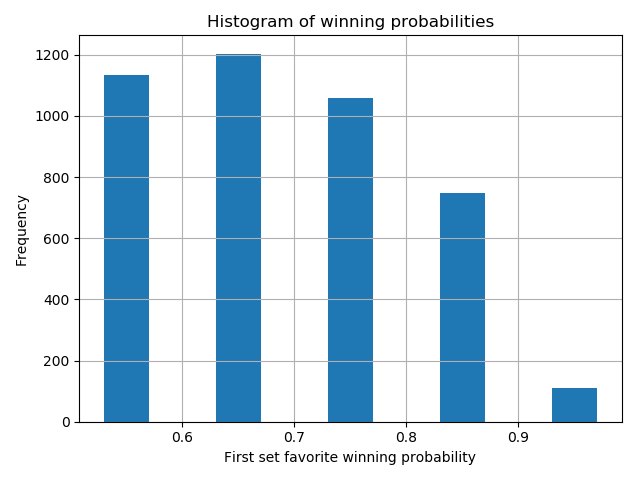
\includegraphics[width=1\textwidth]{C:/Users/1/workspace/mathsport2019/paper/conference_paper/probabilities_histogram}\caption{\label{fig:First-set-winning}First set winning probability $p_{0}$
histogram.}
\par\end{centering}
\end{figure}

\begin{figure}
\begin{centering}
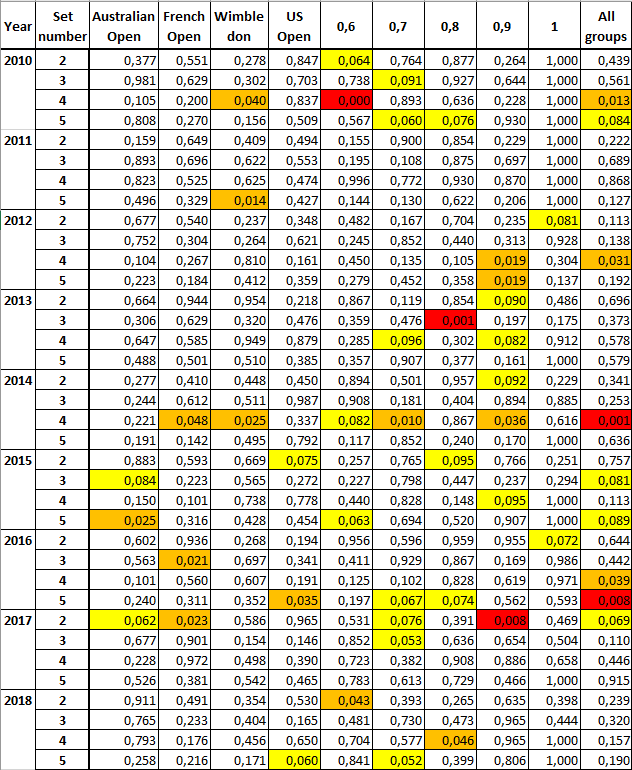
\includegraphics[width=1\textwidth]{C:/Users/1/workspace/mathsport2019/paper/conference_paper/hypothesis_testing.PNG}\caption{\emph{\label{fig:p-values-of-hypothesis}p-values} of hypothesis tests
for different testing sets. Red are marked those allowing to reject
$H_{0}$ on 99\% confidence level, orange on 95\% and yellow on 90\%
confidence level.}
\par\end{centering}
\centering{}
\end{figure}

Overall, the model was tested on 360 different subsets and only 22
of them (6.1\%) provided enough evidence to reject $H_{0}$ on 95\%
confidence level. These subsets are distributed randomly and there
is no pattern among them, indicating there is no systematic bias in
the model. The random walk with varying probabilities thus seems to
be a robust model which can be used to precisely predict set winning
probabilities in men tennis Grand Slam matches.

\section{Test by betting}

The model was implemented and tested in real life setup where it actively
bet in-play against Tipsport, the biggest bookmaker in the Czech Republic.
The test was set up in the following manner.

An automated tool developed using the Python programming language
and Selenium framework running on remote server (Digital Ocean) was
developed and deployed for the purpose of this paper. The tool was
continuously watching odds offering of Tipsport for 2019 men tennis
US Open, especially the set winning odds, and storing the odds into
a database (Postgresql database). Tipsport's starting odds were used
to obtain parameter $p_{0}$ (as described above) and optimized $\lambda$
trained on the 2018 tennis season as the second necessary model parameter.
Every match was observed individually and after each finished set
next set winning probabilities were computed using the presented model.
Whenever the actual set winning odds were higher than the probability
implied odds, i.e. $0>\frac{1}{p}$, a bet was made. The amount betted
was computed as $p\cdot C$, where $C$ was some bankroll dependent
constant (in this case CZK $50$). This amount was further rounded
with precision CZK $1$ (due to betting limitations of Tipsport).
Overall, $131$ bets were made with the total amount CZK $2992$ betted.
$3$ bets were cancelled due to one of the players forfeiting the
match (because of injury). Among these bets the expected number of
wins was $59.85$ whereas the actual number of wins was $57$. The
theoretical expected win with constant bet of $1$ on each bet is
$11.1$ compared to actual theoretical win of $3$ units. The above
mentioned betting system yielded expected win $4.91$ units, and was
actually $2.24$ units.

An automated betting and odds scraping tool was developed using the
Python programming language and Selenium framework. The tool operates
with Tipsport's website and scrapes it for both pre-match as well
as in-play odds. It observes all selected matches (in this case men
tennis US Open matches) and, for the purpose of this study, first
scrapes the first set closing odd, i.e. the last odds available before
the match start. It then observes the match's progress and scrapes
next set winning odds at the moment between to sets to be played.
All these odds are stored into a database, together with some general
information about the match, such as the tournament it is played on,
respective players, starting time etc. Additionally, the model is
applied live and set winning probabilities are calculated on the fly
as are the matches played. Whenever is the set winning probability
higher than the odds implied set winning probability, the tool makes
an actual bet. The bet amount $b$ is set as described above, i.e.
itdepends on the set winning probability $p$, namely $b=p\cdot C,$
where $C$ is some constant (in this particular case CZK $50$ again).


\subsection{Alternative testing}


\section{Concluding remarks\label{sec:Conclusion}}

Neco jako ze to je zajimavy model a ma navic vysledky na live sazeni.

In the present paper, a model of Bernoulli-like random walk with transitions
dependent on the walk history was introduced. Naturally, the model
idea can lead to a more general models, however even a rather simple
version presented here showed a sufficient flexibility, when applied
to tennis matches modelling. First, the fit of the model was tested
statistically, then it was tested also via its use in real in-play
betting, with rather encouraging results.

The source code containing all functionality mentioned in this article
including the automated betting engine is freely available as open
source at GitHub (https://github.com/tomaskourim/mathsport2019) together
with a database containing all data that was used in this paper. Some
results can be also obtained from the same repository.

\section*{Funding}

The research was supported by the grant No. 18-02739S of the Grant
Agency of the Czech Republic.

\bibliographystyle{plain}
\bibliography{C:/Users/1/workspace/mathsport2019/paper/conference_paper/doktknih}

\end{document}
